%!TEX root = report.tex

A convolutional neural network is used as a basis. The activation functions are replaced by Rectified Linear Units. Furthermore is local cost normalization added after the convolution layer and before the max pooling function. 

\begin{table}[ht!]
\centering
\begin{tabular}{ll}
\textbf{Parameter}           & \textbf{Value} \\ \hline  
Learning rate($\eta$) & 0.1   \\
\# of kernels   		& [20 50]   \\
L2 regularization   & 0.0001 \\
Batch Size          & 500     \\
Max epochs          & 200   \\   
\end{tabular}
\caption{The parameters used for the neural network}
\label{parameters2}
\end{table}

The same values as for the base convolutional neural network. These can be seen in Table \ref{parameters2}. The neural network has two convolutional layers with a hidden layers. The hidden layer has 800 inputs with 500 outputs. Finally is there a logistic regression layer which gives 10 outputs, 1 for every digit. The same MNIST handwritten digits dataset was used as for assignment 1.


\begin{figure}[ht!]
	\centering
	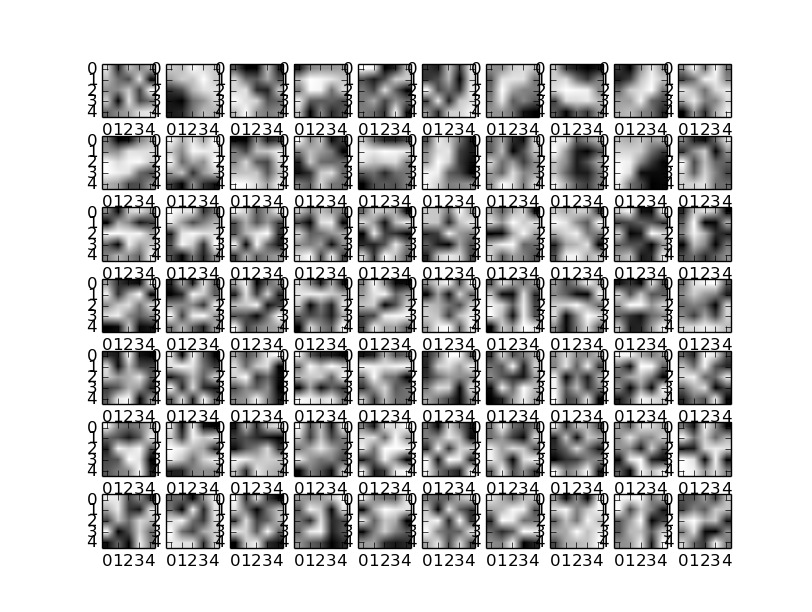
\includegraphics[width=0.9\textwidth]{./img/Exercise2/Afterlearning.png}	
	\caption{The final learned kernels for the convolutional neural network.}
	\label{fig:2:learningKernels}
\end{figure}

\begin{table}[ht!]
\centering
\begin{tabular}{llll}
\textbf{Epoch} & \textbf{Validation error} & \textbf{Test error}\\ \hline
1              & 18.14\%                   & 18.68\%                       \\
49             & 1.58\%                    & 1.58\%                        \\                    
\end{tabular}
\caption{The results for the convolutional neural network.}
\label{results2}
\end{table}

The results can be seen in Table \ref{results2}. The neural network took 52.03 minutes to learn. Since there are 10 classes, the chance for a random correct classification is 10\%, which would mean the test error would be around 90\%. As can be seen in Table \ref{results2}, the resulting test error was 1.58, which is a lot below what the random test error is. 

The Figure \ref{fig:2:learningKernels} shows the 70 kernels. Of which the first 20 kernels show the first layer of the convolutional layer, and the second shows the first 50 for the second layer. The first layer shows clear local contrast, due to the clear borders between the dark and light colours in the graphs.

\todo[inline]{LCN uitleggen}

% best val score 1.58\% at iteration 4900(out of 10000 or 100 epochs), test performance 1.58\%. Took 52.03 minutes.
% Beginning val error was 18.14 and test was 18.68.